\documentclass[../main.tex]{subfiles}
\graphicspath{{\subfix{../images/}}}

\begin{document}

\subsection{Γενική Περιγραφή}
\begin{enumerate}
	\item Οι οντότητες είναι ο \textbf{Χαρακτήρας} (character), ο \textbf{οίκος}
	      (house), τα μη ανθρώπινα \textbf{έμβια όντα} (non human) τα οποία είναι
	      είτε ζωώδη πλάσματα (beast) είτε φυτοειδή (plants), η \textbf{θρησκεία}
	      (religion), και τα \textbf{σημαντικά γεγονότα} στην μυθοπλασία του Game Of Thrones
	      (notable events) .
	\item Για κάθε χαρακτήρα έχουμε πολλές συνδέσεις υποχρεωτικές και μη. Ο
	      χαρακτήρας είναι πιθανό να ανήκει σε έναν οίκο αλλά ένας οίκος είναι
	      υποχρεωτικό να αποτελείται από αυτούς.
	\item Επίσης μπορεί να έχει ένα μη ανθρωποειδές ων στην κατοχή του ή να
	      πιστεύει σε μια θρησκεία.
	\item Δεν είναι υποχρεωτικό να έχει συμμετάσχει σε ένα σημαντικό γεγονός αν
	      και αυτό είναι το πιο πιθανό γιατί κάποια από αυτά θα μπορεί ας πούμε να
	      συνέβησαν μόνο με δράκους (beast).
\end{enumerate}

% ------Table template for entities-------
\newcommand{\entityTable}[4]{
	\renewcommand{\arraystretch}{1.5}
	\tymin 0.25\textwidth
	\begin{table}[H]
		\centering
		\begin{tabulary}{\textwidth}{R|L}
			\hline
			\multicolumn{2}{c}{Οντότητα: \textbf{#1}} \\
			\hline
			\textbf{Περιγραφή}  & #2  \\
			\textbf{Ιδιότητες}  & #3  \\
			\textbf{Γνωρίσματα} & #4  \\
			\hline
		\end{tabulary}
		\caption{Πίνακας οντότητας #1}
		\label{tab:entity_#1}
	\end{table}
}

% ------Table template for relations-------
\newcommand{\relationTable}[6]{
	\renewcommand{\arraystretch}{1.5}
	\tymin 0.3\textwidth
	\begin{table}[H]
		\centering
		\begin{tabulary}{\textwidth}{R|L}
			\hline
			\multicolumn{2}{c}{Οντότητα: \textbf{#1}} \\
			\hline
			\textbf{Περιγραφή}            & #2  \\
			\textbf{Ιδιότητες}            & #3  \\
			\textbf{Λόγος πληθικότητας}   & #4  \\
			\textbf{Συμμετοχή}            & #5  \\
			\textbf{Γνωρίσματα}           & #6  \\
			\hline
		\end{tabulary}
		\StrSubstitute{#1}{\_}{-}[\temp]
		\caption{Πίνακας συσχέτισης \texttt{#1}}
		\label{tab:relation_\temp}
	\end{table}
}

\subsection{Καθορισμός Οντοτήτων}

\entityTable{Character}
{Οντότητα που αποθηκεύονται οι χαρακτήρες}
{Ισχυρή Οντότητα}
{character\_id, name, date\_of\_birth, date\_of\_death, culture, titles}

\entityTable{Fill entities}
{Κάνε copy paste και συμπλήρωσέτα}
{Ισχυρή Οντότητα}
{character\_id, name, date\_of\_birth, date\_of\_death, culture, titles}


\subsection{Καθορισμός Συσχετίσεων}

\relationTable{character\_belongs\_to\_house}
{Κάθε χαρακτήρας μπορεί να έχει έναν οίκο τον οποίο υπηρετεί.}
{belongs-to: διαδική}
{N:1}
{Μερική Συμμετοχή του Character}
{rank}

\subsection{Διάγραμμα Οντοτήτων/Συσχετίσεων}
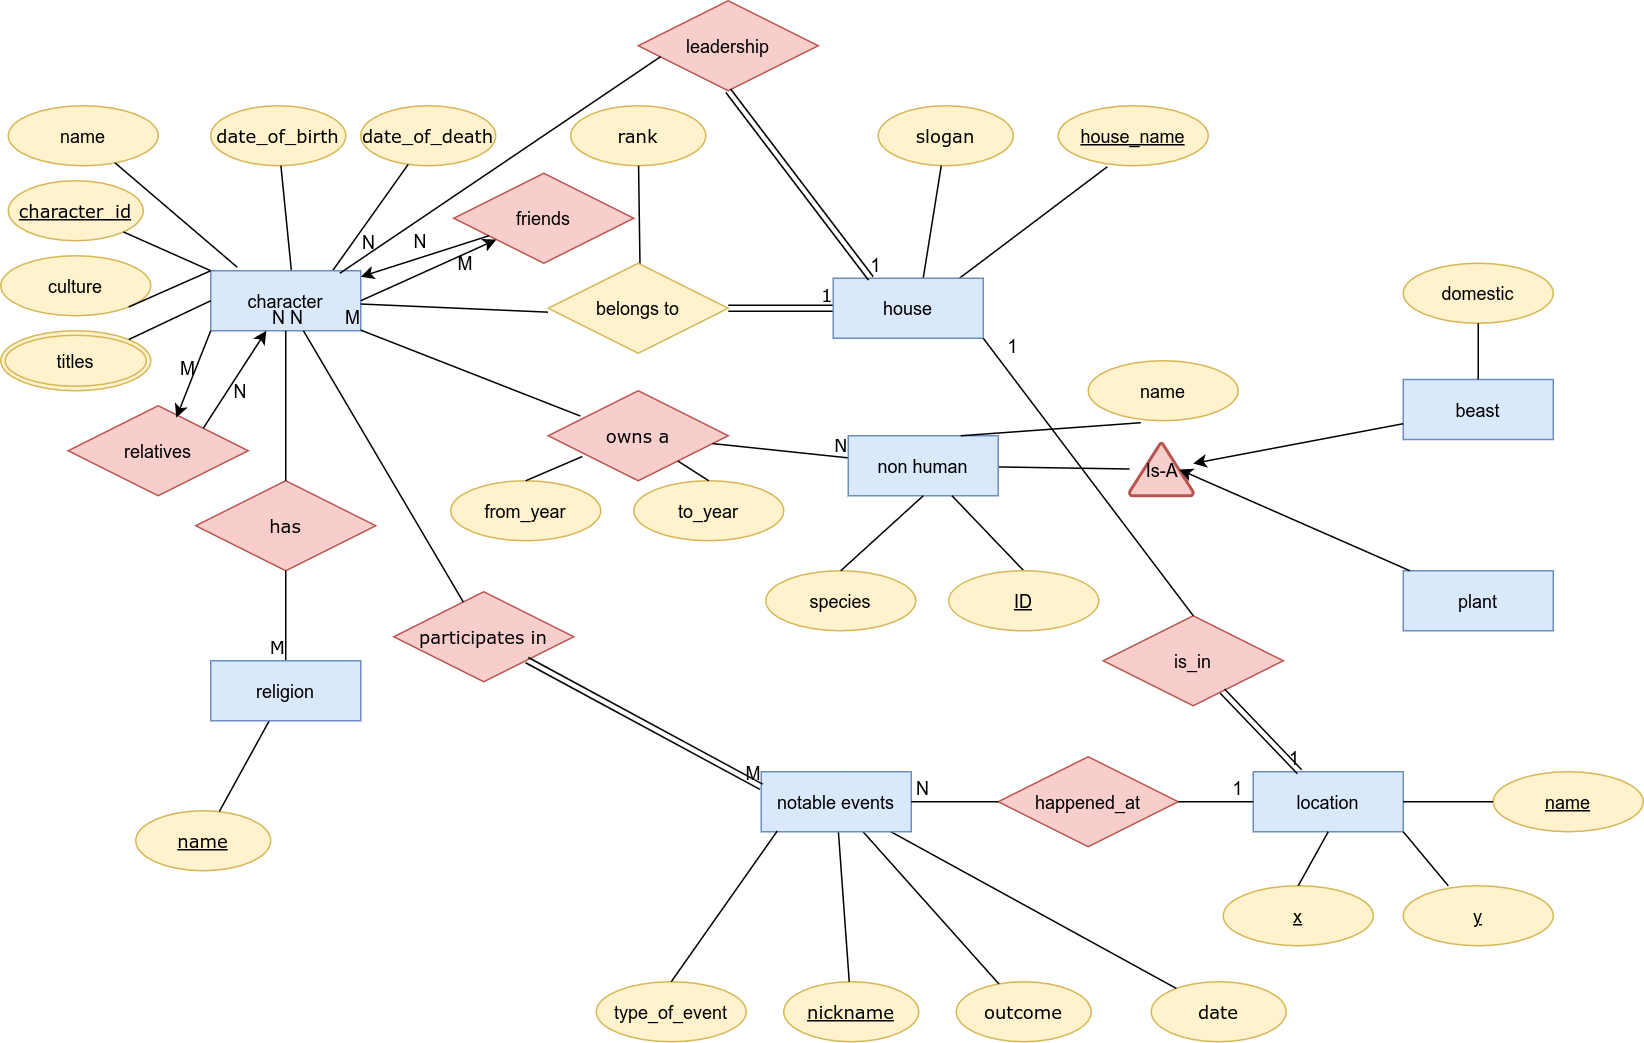
\includegraphics[width=\textwidth]{../images/entity_relation_diagram.png}


\end{document}
